\section{Processing the Dataset}\label{sec:processdataset}

First of the dataset was loaded from \textit{‘.arff’} files using a script that was created, called \textbf{dataio.py}. Each forecasting period have its own file and these datasets can be found in \textit{‘data/’} path. A third party library called \textbf{arff} \cite{python:arff} was used in this script to load the data from files with an \textit{‘.arff’} format. These files were then converted into \textbf{pandas} \cite{python:pandas} dataframes, where an example can be shown in Table \ref{table:pandasex}.

\begin{table}[H]
\centering
  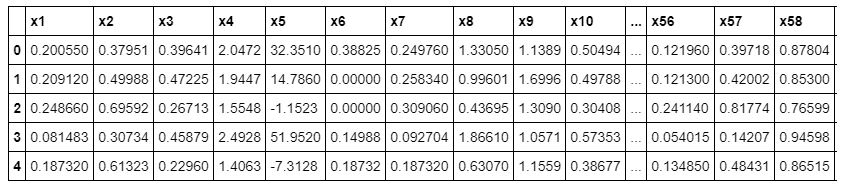
\includegraphics[scale = .65]{imgs/pandas_example_year_1.JPG}
  \caption{An example of a \textbf{pandas'} dataframe for Year 1 }
  \label{table:pandasex}
\end{table}

\noindent Once all the datasets were loaded, the imputation techniques (Mean and Mode) described in Section \ref{sssec:imputetech} were applied. To do so a script was created called \textbf{preprocessing.py} and this script was called from the IPython notebook to apply these techniques. In this script a third party library called \textbf{sklearn.impute} \cite{python:sklearn_api} was utilized to help with the imputation process. The imputation techniques were applied to each forecasting periods and once this process was done they were saved in \textit{‘data/’} path as \textit{‘.arff’} files. A function from the \textbf{preprocessing.py} script was called to do so, and this function uses a third party library \textbf{scipy.io} \cite{python:scipy} to save these files. This was done so the imputation process would be done only once and whenever these imputed datasets are needed, they can be called from the \textit{‘data/’} folder.

\noindent After the imputation techniques were applied, oversampling using SMOTE as described in Subsection \ref{sssec:smote} was applied to each imputed dataset for each forecasting period. A third party library called \textbf{imblearn.over\_sampling} \cite{python:imblearn} was utilized in the \textbf{preprocessing.py} script to apply oversampling. After oversampling, there was a total of 10 different datasets as \textbf{pandas'} dataframes (5 forecasting periods * 2 imputation techniques) and the number of instances almost doubled after this (refer to Table \ref{table:imb_labell} for the original number of instances).

\noindent Following the oversampling process, dimensionality reduction and feature selection techniques described in Section \ref{sec:dimred} were applied. A script called \textbf{feature\_extraction.py} was created for such processes. First an analysis was done to find the number of components to be used in PCA. The first forecasting period (\nth{1} year) in the Mean imputed dataset was used for this analysis, and this was done to get a rough estimate on the number of components to use. A copy of this dataset was standardized as described in Subsection \ref{ssec:standardization}, since the covariance matrix technique will be used. A plot was generated as shown in Figure \ref{fig:pca_analysis} to find the best number of components which keeps as much variance as possible. The best number of components was selected which was 29 components. PCA was then applied to each imputed dataset, for each forecasting period, and the features were reduced to 29 dimensions (the original copy of the datasets were kept since they will be used in the experiments). A third party library \textbf{sklearn.decomposition} \cite{python:sklearn_api} was utilized in \textbf{feature\_extraction.py} to apply PCA. Since the features were reduced to 29, the top 29 features will be selected in Feature Selection techniques, this is done for comparative reasons.
\begin{figure}[H]
\centering
  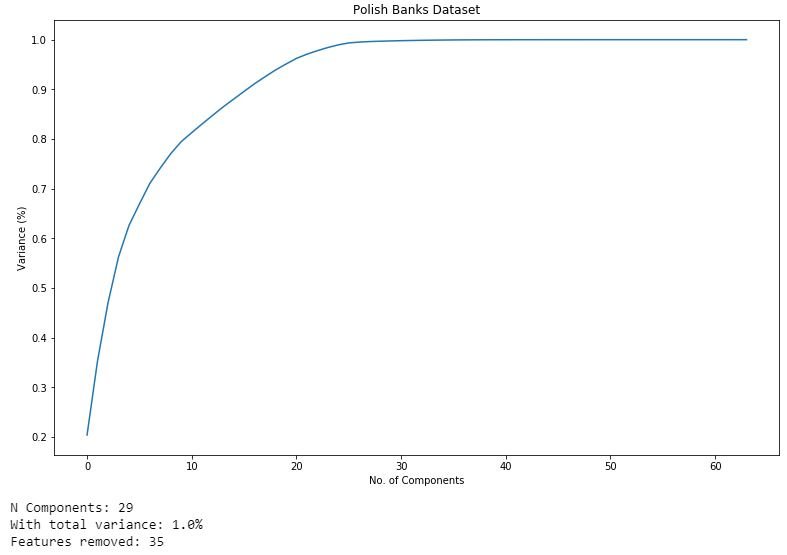
\includegraphics[scale = 0.6]{imgs/pca_analysis.JPG}
  \caption{PCA analysis on Mean Imputed Year 1 forecasting period}
  \label{fig:pca_analysis}
\end{figure}
\noindent Chi2 Feature Selection as described in Subsection \ref{ssec:chisquared} was then applied. Similar to the process for PCA the \nth{1} forecasting period for the Mean Imputed dataset was used to get a rough estimate of the most important features. Since the dataset contains negative values as shown in Subsection \ref{sssec:featmagnitude}, the features were re-scaled using the Equation \ref{eq:normrescale} to the range between 0 and 1 (using \textbf{preprocessing.py} script). The Chi2 statistic score was computed for each feature and the top 29 features were selected as shown in Figure \ref{fig:chisqauredfeat}. A copy of the datasets with these selected features were taken to be used in the experiments. A third party library \textbf{sklearn.feature\_selection} \cite{python:sklearn_api} was utilized in \textbf{feature\_extraction.py} to apply Chi2 Feature Selection. \begin{figure}[H]
\centering
  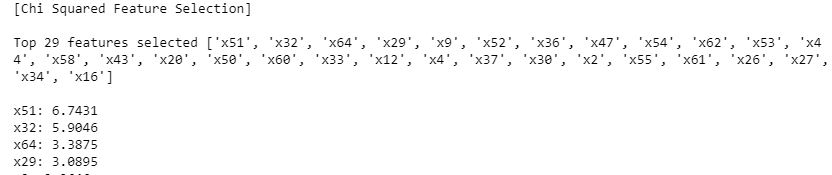
\includegraphics[scale = 0.8]{imgs/chi_squared_feature.JPG}
  \caption{Top features selected using Chi2 based on Year 1 Mean Imputed dataset}
  \label{fig:chisqauredfeat}
\end{figure}
\noindent RFE technique was then applied to select the top 29 features as described in Subsection \ref{ssec:rfe}. Again, as the two previous techniques the two datasets was used to get a rough estimate of the most important features. The Logistic Regression model which was described in Subsection \ref{ssec:logreg} was used as an estimator for this technique and a termination condition of 1000 epochs was used. For the reasons described in Subsection \ref{ssec:normalisation} the dataset was also re-scaled to the range of 0 and 1 to help with gradient descent. The top 29 features selected by this technique are shown in Figure \ref{fig:rfefeat}. A copy of the datasets with these selected features were taken to be used in the experiments. A third party \textbf{sklearn.feature\_selection} \cite{python:sklearn_api} was utilized in \textbf{feature\_extraction.py} to apply RFE. Now that the datasets have been processed, the experiments described in the next section can be conducted.
\begin{figure}[H]
\centering
  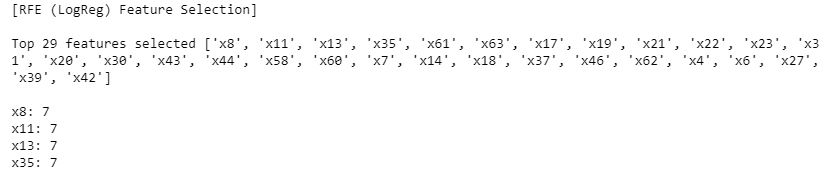
\includegraphics[scale = 0.8]{imgs/rfe_feature.JPG}
  \caption{Top features selected using RFE based on Year 1 Mean Imputed dataset}
  \label{fig:rfefeat}
\end{figure}



